\subsection{平行直线}\label{subsec:1-5}
\begin{enhancedline}

在平面几何里,我们曾学过:“在同一个平面内,如果两条直线都和第三条直线平行,那么这两条直线也互相平行”。
对于空间的三条直线,实际上也有这样的性质,我们把它作为公理。

\begin{gongli}[公理4][gl:zxpx]
    平行于同一条直线的两条直线互相平行。
\end{gongli}

例如,图 \ref{fig:ltjh-1-14} 里三棱镜的三条棱,如果 $AA' \pingxing BB'$、$CC' \pingxing BB'$,
这时必有 $AA' \pingxing CC'$。

\begin{figure}[htbp]
    \centering
    \begin{minipage}[b]{7cm}
        \centering
        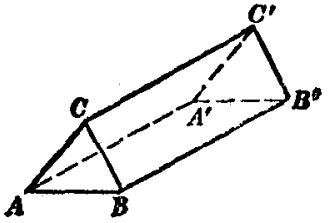
\includegraphics[width=4cm]{../pic/ltjh-ch1-14.png}
        \caption{}\label{fig:ltjh-1-14}
    \end{minipage}
    \qquad
    \begin{minipage}[b]{7cm}
        \centering
        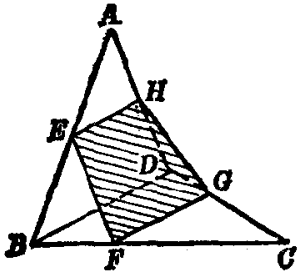
\includegraphics[width=4cm]{../pic/ltjh-ch1-15.png}
        \caption{}\label{fig:ltjh-1-15}
    \end{minipage}
\end{figure}

\liti[0] 已知:四边形 $ABCD$ 是空间四边形(四个顶点不共面的四边形),
$E$、$H$ 分别是边 $AB$、$AD$ 的中点, $F$、$G$ 分别是边 $CB$、$CD$ 上的点,
且 $\dfrac{CF}{CB} = \dfrac{CG}{CD} = \exdfrac{2}{3}$。
求证:四边形 $EFGH$ 是梯形。

\zhengming 如图 \ref{fig:ltjh-1-15},连结 $BD$。

$\because$ \quad $EH$ 是 $\triangle ABD$ 的中位线,

$\therefore$ \quad $EH \pingxing BD$, $EH = \exdfrac{1}{2} BD$。

又在 $\triangle BCD$ 中, $\dfrac{CF}{CB} = \dfrac{CG}{CD} = \exdfrac{2}{3}$,

$\therefore$ \quad $FG \pingxing BD$, $FG = \exdfrac{2}{3} BD$。

根据\nameref{gl:zxpx},$EH \pingxing FG$。

又 $\because$ \quad $FG > EH$,

$\therefore$ \quad 四边形 $EFGH$ 是梯形。

根据\nameref{gl:zxpx},我们可以证明下面的定理:

\begin{dingli}[定理]
    如果一个角的两边和另一个角的两边分别平行并且方向相同,那么这两个角相等。
\end{dingli}

已知: $\angle BAC$ 和 $\angle B'A'C'$ 的边 $AB \pingxing A'B'$, $AC \pingxing A'C'$,并且方向相同。

求证: $\angle BAC = \angle B'A'C'$。

\zhengming 对于 $\angle BAC$ 和 $\angle B'A'C'$ 都在同一平面内的情况,
在平面几何中已经证明。下面我们证明两个角不在同一平面内的情况。

如图 \ref{fig:ltjh-1-16},在 $AB$、$A'B'$,$AC$、$A'C'$ 上分别取 $AD = A'D'$、
$AE = A'E'$,连结 $AA'$、$DD'$、$EE'$、$DE$、$D'E'$。

\begin{wrapfigure}[8]{r}{5cm}
    \centering
    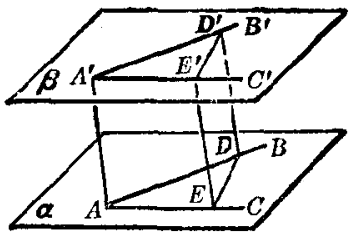
\includegraphics[width=5cm]{../pic/ltjh-ch1-16.png}
    \caption{}\label{fig:ltjh-1-16}
\end{wrapfigure}

$\because$ \quad $AB \pingxing A'B'$, $AD = A'D'$,

$\therefore$ \quad $AA'D'D$ 是平行四边形。

$\therefore$ \quad $AA' \pxqdy DD'$。

同理 \quad $AA' \pxqdy EE'$。

根据\nameref{gl:zxpx} 得 $DD' \pingxing EE'$。

又可得  $DD' = EE'$,

$\therefore$ \quad 四边形 $EE'D'D$ 是平行四边形。

$\therefore$ \quad $ED = E'D'$。 可得 $\triangle ADE \quandeng \triangle A'D'E'$。

$\therefore$ \quad $\angle BAC = \angle B'A'C'$。

把上面两个角的两边反向延长,就得出下面的推论:

\begin{tuilun}[推论]
    如果两条相交直线和另两条相交直线分别平行,那么这两组直线所成的锐角(或直角)相等。
\end{tuilun}

\zhuyi 由上面定理的证明可知:平面里的定义、定理等,对于非平面图形,需要经过证明才能应用。


\begin{lianxi}

\xiaoti{把一张长方形的纸对折两次,打开后如图那样,说明为什么这些折痕是互相平行的。}

\begin{figure}[htbp]
    \centering
    \begin{minipage}[b]{7cm}
        \centering
        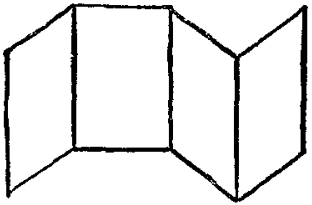
\includegraphics[width=5cm]{../pic/ltjh-ch1-subsec5-lx-01.png}
        \caption*{(第 1 题)}
    \end{minipage}
    \qquad
    \begin{minipage}[b]{7cm}
        \centering
        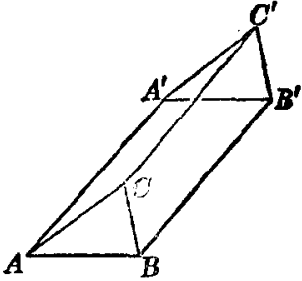
\includegraphics[width=4cm]{../pic/ltjh-ch1-subsec5-lx-02.png}
        \caption*{(第 2 题)}
    \end{minipage}
\end{figure}

\xiaoti{已知:如图, $AA'$、$BB'$、$CC'$ 不共面,且 $BB' \pxqdy AA'$, $CC' \pxqdy AA'$。
    求证: $\triangle ABC \quandeng \triangle A'B'C'$。
}

\end{lianxi}

\end{enhancedline}
